\documentclass[11pt]{article} 

\usepackage[utf8]{inputenc} 

%%% PAGE DIMENSIONS
\usepackage{geometry} % to change the page dimensions
\geometry{a4paper} % or letterpaper (US) or a5paper or....
\geometry{margin=1in} % for example, change the margins to 2 inches all round

\usepackage{graphicx} % support the \includegraphics command and options

%%% PACKAGES
\usepackage{booktabs} % for much better looking tables
\usepackage{array} % for better arrays (eg matrices) in maths
\usepackage{paralist} % very flexible & customisable lists (eg. enumerate/itemize, etc.)
\usepackage{verbatim} % adds environment for commenting out blocks of text & for better verbatim
%\usepackage{subfig} % make it possible to include more than one captioned figure/table in a single float
\usepackage{enumitem}
\usepackage{multicol}
\usepackage{tikz}
\usepackage{subcaption}
\usepackage{multirow}
\usepackage[brazilian]{babel}
\usepackage[siunitx]{circuitikz}
\tikzset{
  declare function={% in case of CVS which switches the arguments of atan2
    atan3(\a,\b)=ifthenelse(atan2(0,1)==90, atan2(\a,\b), atan2(\b,\a));},
  kinky cross radius/.initial=+.125cm,
  @kinky cross/.initial=+, kinky crosses/.is choice,
  kinky crosses/left/.style={@kinky cross=-},kinky crosses/right/.style={@kinky cross=+},
  kinky cross/.style args={(#1)--(#2)}{
    to path={
      let \p{@kc@}=($(\tikztotarget)-(\tikztostart)$),
          \n{@kc@}={atan3(\p{@kc@})+180} in
      -- ($(intersection of \tikztostart--{\tikztotarget} and #1--#2)!%
             \pgfkeysvalueof{/tikz/kinky cross radius}!(\tikztostart)$)
      arc [ radius     =\pgfkeysvalueof{/tikz/kinky cross radius},
            start angle=\n{@kc@},
            delta angle=\pgfkeysvalueof{/tikz/@kinky cross}180 ]
      -- (\tikztotarget)}}}

%%% HEADERS & FOOTERS
\usepackage{fancyhdr} % This should be set AFTER setting up the page geometry
\pagestyle{fancy} % options: empty , plain , fancy
\renewcommand{\headrulewidth}{0pt} % customise the layout...
\lhead{}\chead{Universidade Federal Fluminense\\Departamento de Engenharia Elétrica\\TEE00129 - Laboratório de Eletrônica Básica}\rhead{}
\lfoot{}\cfoot{\thepage}\rfoot{}

%%% SECTION TITLE APPEARANCE
%\usepackage{sectsty}
%\allsectionsfont{\sffamily\mdseries\upshape} % (See the fntguide.pdf for font help)

%%% ToC (table of contents) APPEARANCE
\usepackage[nottoc,notlof,notlot]{tocbibind} % Put the bibliography in the ToC
\usepackage[titles,subfigure]{tocloft} % Alter the style of the Table of Contents
\renewcommand{\cftsecfont}{\rmfamily\mdseries\upshape}
\renewcommand{\cftsecpagefont}{\rmfamily\mdseries\upshape} % No bold!

%%% END Article customizations

\title{Aula 4: Transistores Bipolares}
\author{Prof. Derick Furquim Pereira}
\date{} % Activate to display a given date or no date (if empty),
         % otherwise the current date is printed 

\begin{document}
\maketitle
\thispagestyle{fancy}

\section*{Parte teórica}

\subsection*{Questionário}

\begin{enumerate}

\item (4,0) Dado o circuito abaixo, encontre os valores de $V_B$, $V_C$, $V_E$, $I_B$, $I_C$ e $I_E$. Considere $\beta=300$ e $V_{BE}=0,7$ V.
\begin{figure}[!h]
	\centering
	\begin{circuitikz}[american voltages,scale=.7, transform shape]
	\draw
	% Drawing a npn transistor
	(0,0) node[npn](npn1){}
	% Making connections from transistor using relative coordinates
	(npn1.B) -- ++(-1,0) node(base){}
	(npn1.B) -- ++(-1,0) to [R,l=10<\kilo\ohm>,*-] ++(0,3) node(con1){}
	(0,3) node(con2){}
	(npn1.B) -- ++(-1,0) to [R,l_=2.2<\kilo\ohm>,*-] ++(0,-3) node(gnd1){}
	(npn1.E) to [R,l=330<\kilo\ohm>,i=$I_E$,*-] (0,-3)
	(con2) to [R,l=1<\kilo\ohm>,i>^=$I_C$,-*] (npn1.C)
%	(npn1.C) to [R,l_=1<\kilo\ohm>,i=$i_C$,*-] (0,3)
	% Drawing shorts and ground connection
	(0,3)to[short,*-o] (0,4) node[right]{$V_{CC}=10 V$} % Power supply
	(0,-3) node[ground]{}% Define this node as ground
	(gnd1) ++(0,0) to[short,-*] ++(1.85,0)
	(con1)to[short] ++(1.85,0)
	(base) to[short,i=$I_B$] ++(1,0)
	(npn1.C) node[anchor=west]{C}
	(base) node[anchor=east]{B}
	(npn1.E) node[anchor=west]{E}
	;
	\end{circuitikz}
	\caption{Circuito de polarização do BJT por divisor de tensão.}
\end{figure}

\end{enumerate}

\section*{Verificação do ganho DC do transistor}

\subsection*{Procedimento}

Coloque as chaves S2, S3 e S4 do \textit{DIP Switch} na posição fechada (ON) e mantenha as demais chaves na posição aberta. Nesta condição, tem-se o circuito equivalente mostrado na Figura \ref{circ1}.

\begin{figure}[!htb]
\centering
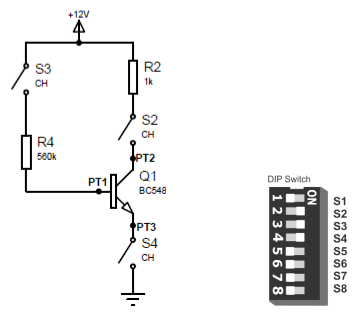
\includegraphics[width=.4\textwidth]{GanhoDC.png}
\caption{Circuito para observar as características de transferência.}
\label{circ1}
\end{figure}

\subsection*{Questionário}

\begin{enumerate}
\setcounter{enumi}{1}
\item (0,75) Com o auxílio de um multímetro, meça e anote os valores de $V_{BE}$ e $V_{CE}$ do circuito mostrado na Figura \ref{circ1}.

\item (0,75) Com base nas medições realizadas na questão anterior, calcule os valores de $I_B$, $I_C$ e $\beta$ do transistor Q1 da Figura \ref{circ1}.

\item (0,75) Para o circuito da Figura \ref{circ1}, calcule os extremos, superior e inferior, da reta de carga.
\end{enumerate}

\section*{Transistor como chave}

\subsection*{Procedimento}

Coloque a chave S4 do \textit{DIP Switch} na posição fechada (ON) e mantenha as demais chaves na posição aberta. Nesta condição, tem-se o circuito equivalente mostrado na Figura \ref{circ2}.

\begin{figure}[!htb]
\centering
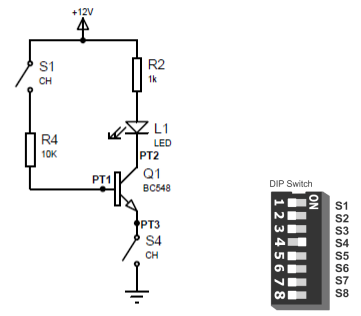
\includegraphics[width=.4\textwidth]{Chave.png}
\caption{Circuito de transistor como chave.}
\label{circ2}
\end{figure}

Abra e feche sucessivamente a chave S1. O LED deve acender e apagar devido à polarização da junção base-emissor, através de R4 e S1, que leva o transistor para o corte e saturação, provocando o chaveamento eletrônico do coletor.

\subsection*{Questionário}

\begin{enumerate}
\setcounter{enumi}{4}

\item (0,75) Com o auxílio de um multímetro, meça e anote o valor da tensão $V_{CE}$, do circuito da Figura \ref{circ2}, para as condições de chave fechada e chave aberta.

\item (0,75) Com base nas medições realizadas na questão anterior, calcule o valor da corrente no coletor do transistor Q1 da Figura \ref{circ2}, para as condições de chave fechada e chave aberta.

\end{enumerate}

\section*{Polarização por divisor de tensão}

\subsection*{Procedimento}

Coloque as chaves S6 e S7 do \textit{DIP Switch} na posição fechada (ON) e mantenha as demais chaves na posição aberta. Ligue a fonte variável do módulo através da chave CH7, e através do potenciômetro +VAR, ajuste a tensão no voltímetro do módulo para +10 V. Nesta condição, tem-se o circuito equivalente mostrado na Figura \ref{circ3}.

\begin{figure}[!htb]
\centering
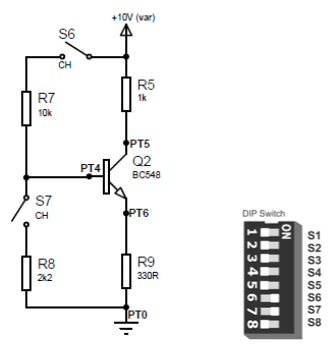
\includegraphics[width=.4\textwidth]{DivisorTensao.png}
\caption{Circuito de polarização por divisor de tensão.}
\label{circ3}
\end{figure}

\subsection*{Questionário}

\begin{enumerate}
\setcounter{enumi}{6}

\item (0,75) Com o auxílio de um multímetro, meça e anote os valores das tensões $V_B$, $V_C$ e $V_E$, do circuito da Figura \ref{circ3}.

\item (0,75) Com base nas medições realizadas na questão anterior, calcule os valores da corrente no coletor ($I_C$) e da tensão $V_{CE}$, do transistor Q1 da Figura \ref{circ3}.

\item (0,75) Compare os resultados das duas questões anteriores com o resultado da parte teórica (Questão 1) do relatório.

\end{enumerate}

\end{document}
